%\documentclass[aspectratio=169, handout]{beamer}
\documentclass[aspectratio=169]{beamer}


\makeatletter
\renewcommand*\env@matrix[1][\arraystretch]{%
  \edef\arraystretch{#1}%
  \hskip -\arraycolsep
  \let\@ifnextchar\new@ifnextchar
  \array{*\c@MaxMatrixCols c}}
\makeatother

\usepackage{tikz}
\usetikzlibrary{tikzmark,fit,shapes.geometric}

\newcommand{\transp}{^{\rm{T}}}

\usepackage{cases}
\usepackage[english]{babel}
% or whatever
\usepackage{xcolor}
\usepackage{colortbl}
\usepackage[latin1]{inputenc}
\usepackage[super]{nth}
% or whatever
%\setbeamertemplate{footline}[page number]
\setbeamertemplate{footline}
        {
      \leavevmode%
      \hbox{%
      \begin{beamercolorbox}[wd=.333333\paperwidth,ht=2.25ex,dp=1ex,center]{author in head/foot}%
        \usebeamerfont{author in head/foot}\insertshortauthor%~~(\insertshortinstitute)
      \end{beamercolorbox}%
      \begin{beamercolorbox}[wd=.333333\paperwidth,ht=2.25ex,dp=1ex,center]{title in head/foot}%
        \usebeamerfont{title in head/foot}\insertshorttitle
      \end{beamercolorbox}%
      \begin{beamercolorbox}[wd=.333333\paperwidth,ht=2.25ex,dp=1ex,right]{date in head/foot}%
        \usebeamerfont{date in head/foot}\insertshortdate{}\hspace*{2em} \insertframenumber{}  \hspace*{2em}%/ \inserttotalframenumber\hspace*{2ex} 

    %#turning the next line into a comment, erases the frame numbers
        

      \end{beamercolorbox}}%
      \vskip 0pt%
    }

\usepackage{times}
\usepackage[T1]{fontenc}
\usepackage{psfrag}
\usepackage{algorithm}
\usepackage{amsmath}
\usepackage{amssymb}
\usepackage{tabularx}
\usepackage{algpseudocode}
\usepackage{mathrsfs}
\usepackage{textpos}
\usepackage{graphicx}
\usepackage{tcolorbox}
\usepackage{multicol}
\usepackage{tikz}
\usetikzlibrary{arrows.meta,shapes.arrows}
%\setkeys{Gin}{draft}
\usepackage{caption}
\captionsetup{font=scriptsize,labelfont=scriptsize}
\usepackage{color}
\DeclareCaptionFont{blue}{\color{blue}}
\captionsetup{labelfont=blue}
\usepackage{tikz}
\tikzset{
  every overlay node/.style={
    draw=white,anchor=north west,
  },
}
\def\checkmark{\tikz\fill[scale=0.4](0,.35) -- (.25,0) -- (1,.7) -- (.25,.15) -- cycle;}
\def\tikzoverlay{%
   \tikz[baseline,overlay]\node[every overlay node]
}%
%\DeclareGraphicsRule{.png}{png}{.png.bb}{}

\newtheorem{assumption}{Assumption} %jw

\newcommand{\T}{{\rm T}}

\newcommand\blfootnote[1]{%
  \begingroup
  \renewcommand\thefootnote{}\footnote{#1}%
  \addtocounter{footnote}{-1}%
  \endgroup
}
\setcounter{tocdepth}{1}
\beamertemplatenavigationsymbolsempty


\title[Lecture 10: Multiple Regression] % (optional, use only with long paper titles)
{Data, Environment and Society: \\{Lecture 10: Multiple Regression}}


%\subtitle
%{Include Only If Paper Has a Subtitle}

\author[ER131: Data, Environment and Society] 
{Instructor: Duncan Callaway\\
GSI: Salma Elmallah} 
% - Give the names in the same order as the appear in the paper.
% - Use the \inst{?} command only if the authors have different
%   affiliation.

%\logo{
%\includegraphics[width=1.5cm,height=1.5cm,keepaspectratio]{uvic_logo_h.jpg}
%}
\vspace{-20mm}
\institute[UC Berkeley] % (optional, but mostly needed)
 {\small{ \bf October 1, 2019}}


\date[October 1, 2019]


\begin{document}

\begin{frame}[plain, noframenumbering]
  \titlepage
\end{frame}

\begin{frame}{Today}

\begin{itemize}
\item First: Finish reviewing Jupyter notebook on confidence intervals.
\begin{itemize}
  \item Objective: understand how a distribution of parameter values is possible when you train OLS with a sample from a population.  
\end{itemize}
\item Next: slides, covering multiple regression and (one form of) model selection.  Slides in GitHub
\begin{itemize}
  \item Model selection is the method for dealing with bias-variance tradeoff
  \item It is one of the most important processes we do in statistical learning  
\end{itemize}
\item Third: Introduction to land use regression, start working with NO2 data in Jupyter notebook
\begin{itemize}
  \item We'll begin learning about a paper that uses one form of model selection.
  \item Later in the semester you'll use the tools from this class to improve on this paper.
\end{itemize}
\end{itemize}

\end{frame}

\begin{frame}{Announcements}
\textbf{Reading}
\begin{itemize}
\item Today: ISLR 3.2
\item Thursday: ISLR Ch 3.3.
\item Next Tuesday: Novotny \textit{et al}, see questions in GitHub folder for lecture 12 reading.
\end{itemize}

\textbf{Survey posted!  Please respond}
\end{frame}


\begin{frame}{Final project -- team and initial idea due Thursday}

\begin{itemize}
\item You can work with your own data
\item But we have also suggested data sets
\item Working in groups up to three ok (you can self-organize)
\item We will give you basic guardrails on what to do
\begin{itemize}
\item Pose a coherent question that can be addressed using the skills we are learning
\item EDA and visualization requirements
\item Carry out multiple prediction exercises using the tools we are learning.
\item Critique the performance of your models
\item Interpret your results within the confines of what your models are capable of.
\end{itemize}
\end{itemize}

\end{frame}

\begin{frame}{What if the confidence interval contains zero?}

For example, if
   
\begin{align*}
  -10.3 < \beta_1 < 24.8?
\end{align*}

...where the upper and lower bounds comprise the 95\% confidence interval.

\pause

\vspace{5mm}
This implies there is more than a remote chance that there is no significant relationship between the dependent and independent variables.  

\end{frame}

%%%%%%%%%%%%%
\begin{frame}{p-values}

\textbf{What are they?}  \pause p-values measure the probability that the estimated coefficients arose by chance from a data generating process that actually has \textit{no} relationship between the inputs and outputs.  

\vspace{5mm}

$p = 0.05$ implies a 5\% chance that the true parameter value is \textit{zero}.  

\vspace{5mm}

If $p\ll0.05$, then the parameter is strongly inside the 95\% confidence interval.

\vspace{5mm}

If $p>0.05$, then the parameter is outside the 95\% confidence interval.

\vspace{5mm}

A small p-value indicates that it is unlikely to observe such a substantial association between the predictor and the response due to chance.

\end{frame}

%%%%%%%%%%%%%
\begin{frame}{p-hacking?}

What's wrong with these practices:
\begin{itemize}
  \item Stop collecting data once $p<0.05$
  \item Analyze many independent variables, but only report those for which $p<0.05$
  \item Collect and analyze many data samples, but only report those with $p<0.05$
  \item Exclude participants to get  $p<0.05$.
  \item Transform the data to get  $p<0.05$.
\end{itemize}

(credit to Leif Nelson, UCB Haas)

\end{frame}

%%%%%%%%%%%%%
\begin{frame}{The trouble with p-hacking...}

...is that by looking for the data set and the models that give low p-values, you could just be looking for those 5\% ``chances'' where the real relationship is non-existent.

\vspace{5mm}

In other words, if you flip a coin with 5\% probability it'll turn up heads enough times, eventually you get heads.

\vspace{5mm}

In the case of p-hacking, a getting a p-value of 5\% when there really is no relationship is the analogy to getting heads on that 5\% probability coin.
\vspace{5mm}
\pause

Some estimates suggest that this practice leads to false positive rates of 61\%!

\end{frame}


\begin{frame}{The origins of p-hacking}

Why do people do it?

\pause 

\vspace{5mm}
\textbf{One explanation:}  Researchers are deliberately deceiving their peers.  They want good results so they go fisihing for them.

\pause
\vspace{5mm}

\textbf{Maybe, but...} 
\begin{itemize}
  \item perhaps people simply don't understand the idea that their parameters are one draw from a \textit{distribution} of possible parameters
  \item and therefore they don't really understand how to interpret $p$.
\end{itemize}

\vspace{5mm}

Now you understand -- so my hope is that you'll always interpret these with caution!
\end{frame}

%%%%%%%%%%%%%
\begin{frame}{Model accuracy: R$^2$}

TSS = total sum of squares

\vspace{3mm}

RSS = residual sum of squares

  \begin{align*}
    R^2 = \frac{TSS - RSS}{TSS} \onslide<2->{= \frac{\sum_{i=1}^n (y_i-\bar{y})^2 - \sum_{i=1}^n e_i^2}{\sum_{i=1}^n (y_i-\bar{y})^2}}\onslide<3->{ = 1-\frac{\sum_{i=1}^n e_i^2}{\sum_{i=1}^n (y_i-\bar{y})^2} }
  \end{align*}

  \pause\pause
  $R^2$ measures the fraction of variation in the dependent variable that is captured by the model.  

\pause
\vspace{5mm}

It's good for capturing predictive power, but not for evaluating the significance of the model.

\end{frame}


\begin{frame}{Let's be clear...}

What do people doing prediction care about, $\hat{\beta}$ or $\hat{y}$?

\vspace{5mm}
\pause

$\hat{y}$!

\vspace{5mm}
\pause

What measure should people doing prediction use to evaluate model performance, coefficient confidence intervals, RSS, R$^2$ or $p$?

\vspace{5mm}
\pause

RSS or R$^2$ are suitable.  But there is much more to the story! 
\begin{itemize}
  \item Today we'll talk about adjustments to R$^2$ that attempt to address bias-variance tradeoff
  \item  We'll discuss other approaches in the coming weeks.
\end{itemize}

\end{frame}

\begin{frame}{Multivariate regression}

This is exactly the same process as single (independent) variable regression: minimize mean squared error (MSE).  Parameter solutions can be found by
\begin{itemize}
\item Gradient search
\item Normal equations
\item Setting partial derivatives of MSE to zero and solving -- but now for $\beta_0, \beta_1, \beta_2,\ldots,\beta_d$ ($d$ is the number of features, a.k.a. independent variables).
\end{itemize}

\vspace{5mm}
The mechanics of finding parameters is easy.  The real challenge is: Which features to include?
\end{frame}

\begin{frame}{Model selection}

\textbf{The challenge:} Don't include variables in your model that lead to over-fit.

\vspace{-5mm}

\begin{figure}
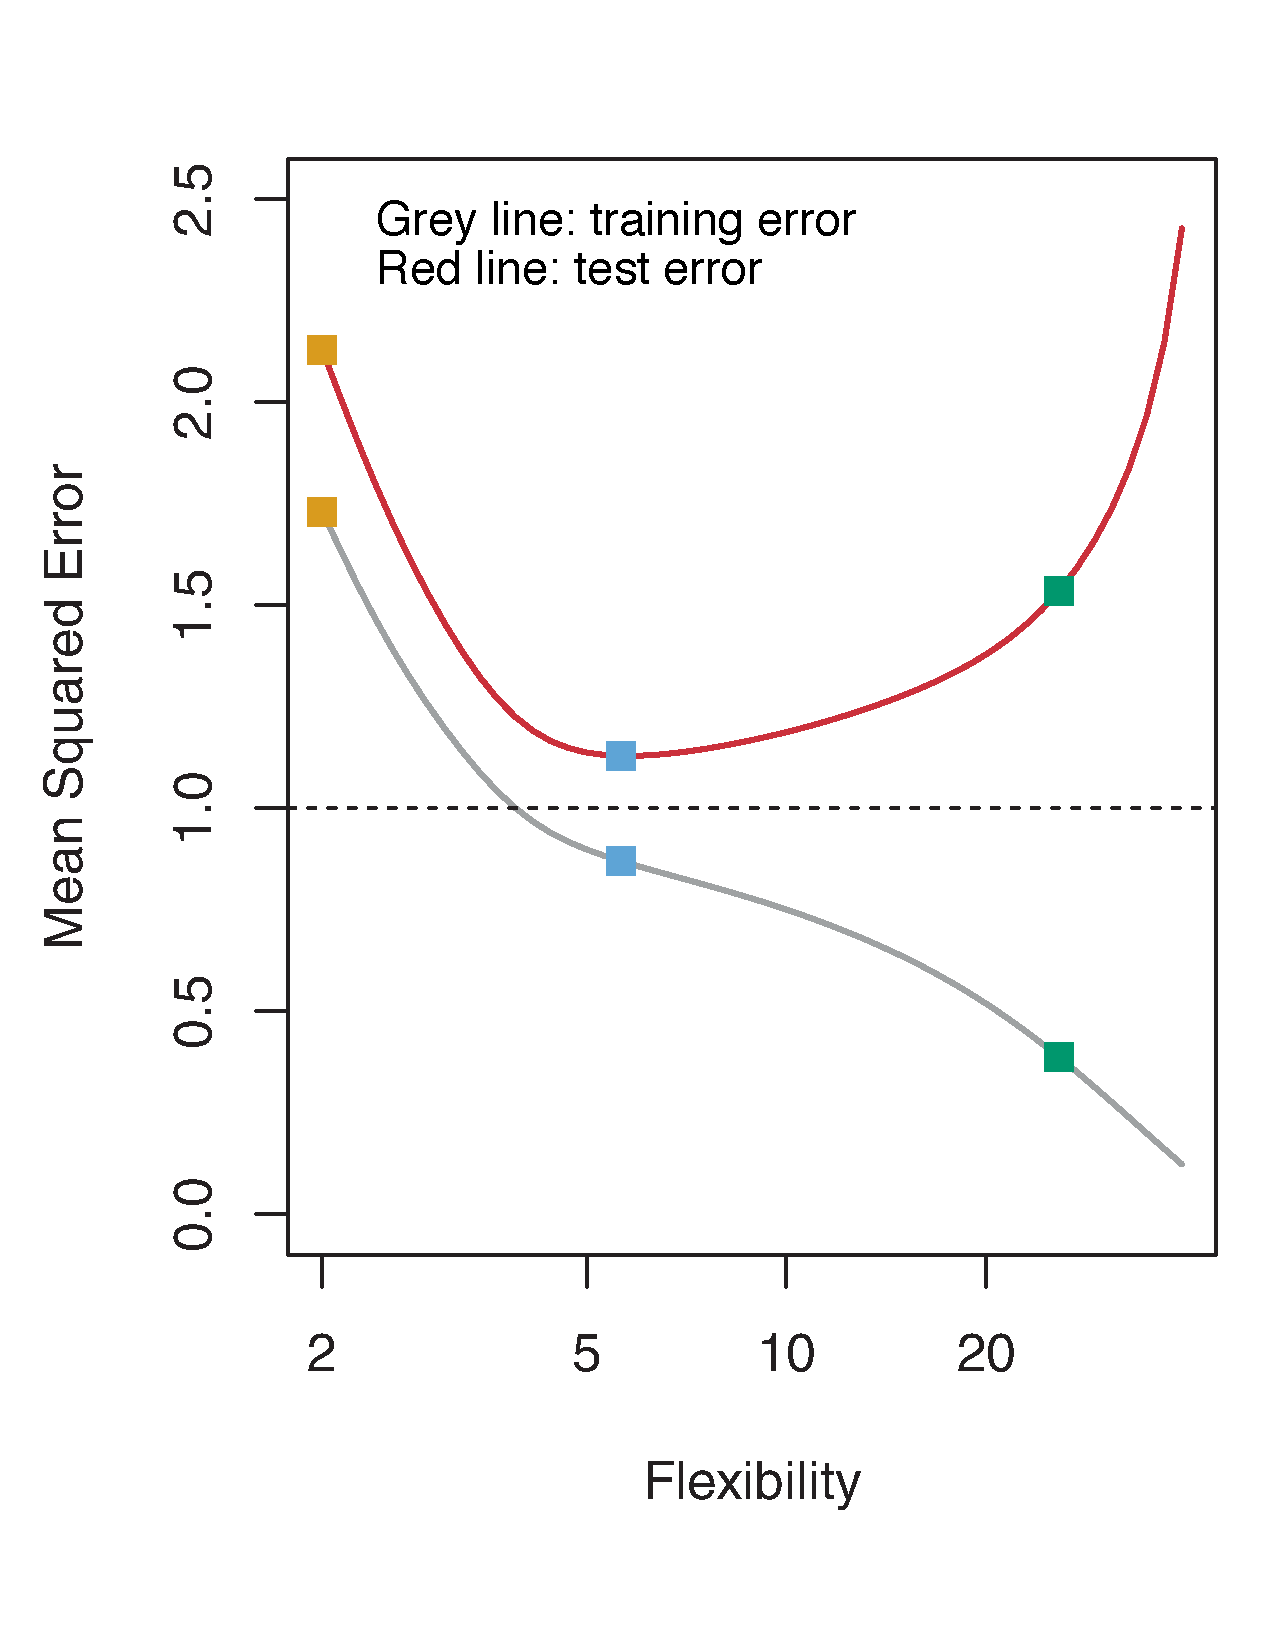
\includegraphics[height=0.8\textheight]{islr2_9b}
\end{figure}

\vspace{-10mm}
With multiple regression, increasing the number of variables increases the flexibility of the model.

\end{frame}

\begin{frame}{Model selection methods}

\textbf{Two basic methods:}
\vspace{5mm}
\begin{itemize}
\item Computationally heavy and theoretically robust: 
\begin{itemize}
\item repeated sampling of train and test data sets
\item build and test models with each sampled set
\item choose the model form that minimizes test error, on average.
\item the figure on the previous slide is an example of this approach.
\end{itemize}
\vspace{5mm}
\item Easy to implement (no need for significant computing):
\begin{itemize}
\item Use the full data set
\item Fit each candidate model once
\item Choose the model that minimizes an ``adjusted'' measure of R2 or mean squared error.
\end{itemize}
\end{itemize}
\end{frame}

\begin{frame}{An easy-to-implement method}

Akaike information criterion (AIC):

\begin{enumerate}
\item Construct all the models you have time for using \textit{all} the data (i.e. all your observations) to train the models.
\item Then, choose the model with the lowest AIC, where
\begin{align*}
\text{AIC} = \frac{1}{n\hat{\sigma}^2}(\text{RSS}+2d\hat{\sigma}^2) \onslide<2->{= \frac{1}{\hat{\sigma}^2}\left(\frac{\text{RSS}}{n}\right) + \frac{2d}{n}}
\end{align*}
\end{enumerate}

$\hat{\sigma}$ is an estimate of the variance of the error $\epsilon$.

\pause
\vspace*{5mm}
As you can see, AIC ``penalizes'' models with a high value of $d$.  
\end{frame}

\begin{frame}{What the heck is AIC?}

It actually has a rigorous theoretical underpinning.  Understanding the derivation requires background in information theory and more time than we have here.  

\vspace{5mm}
\pause

But:
\begin{itemize}
\item It gives unbiased estimate of the MSE you'd get if you \textit{did }use a test data set (as long as the errors are Gaussian)
\item It's ok to just work with the intuition that choosing models that minimize AIC is analogous to 
\begin{itemize}
\item choosing models that minimize MSE ...
\item plus a penalty for the number of features.
\end{itemize}
\end{itemize}

\end{frame}



\begin{frame}{Prediction application: Land use regression}
  \begin{itemize}
    \item Suppose we'd like to know pollutant concentrations at a fine spatial resolution
    \item We only have pollutant measurements at low resolution (coarse spatial scale)
    \item But we have other measurements at finer spatial resolution
    \item This is an ideal job for forecasting.  
    \item But rather than forecast in \textit{time} we will forecast in \textit{space}.
  \end{itemize}

\begin{columns}
\column{0.75\textwidth}
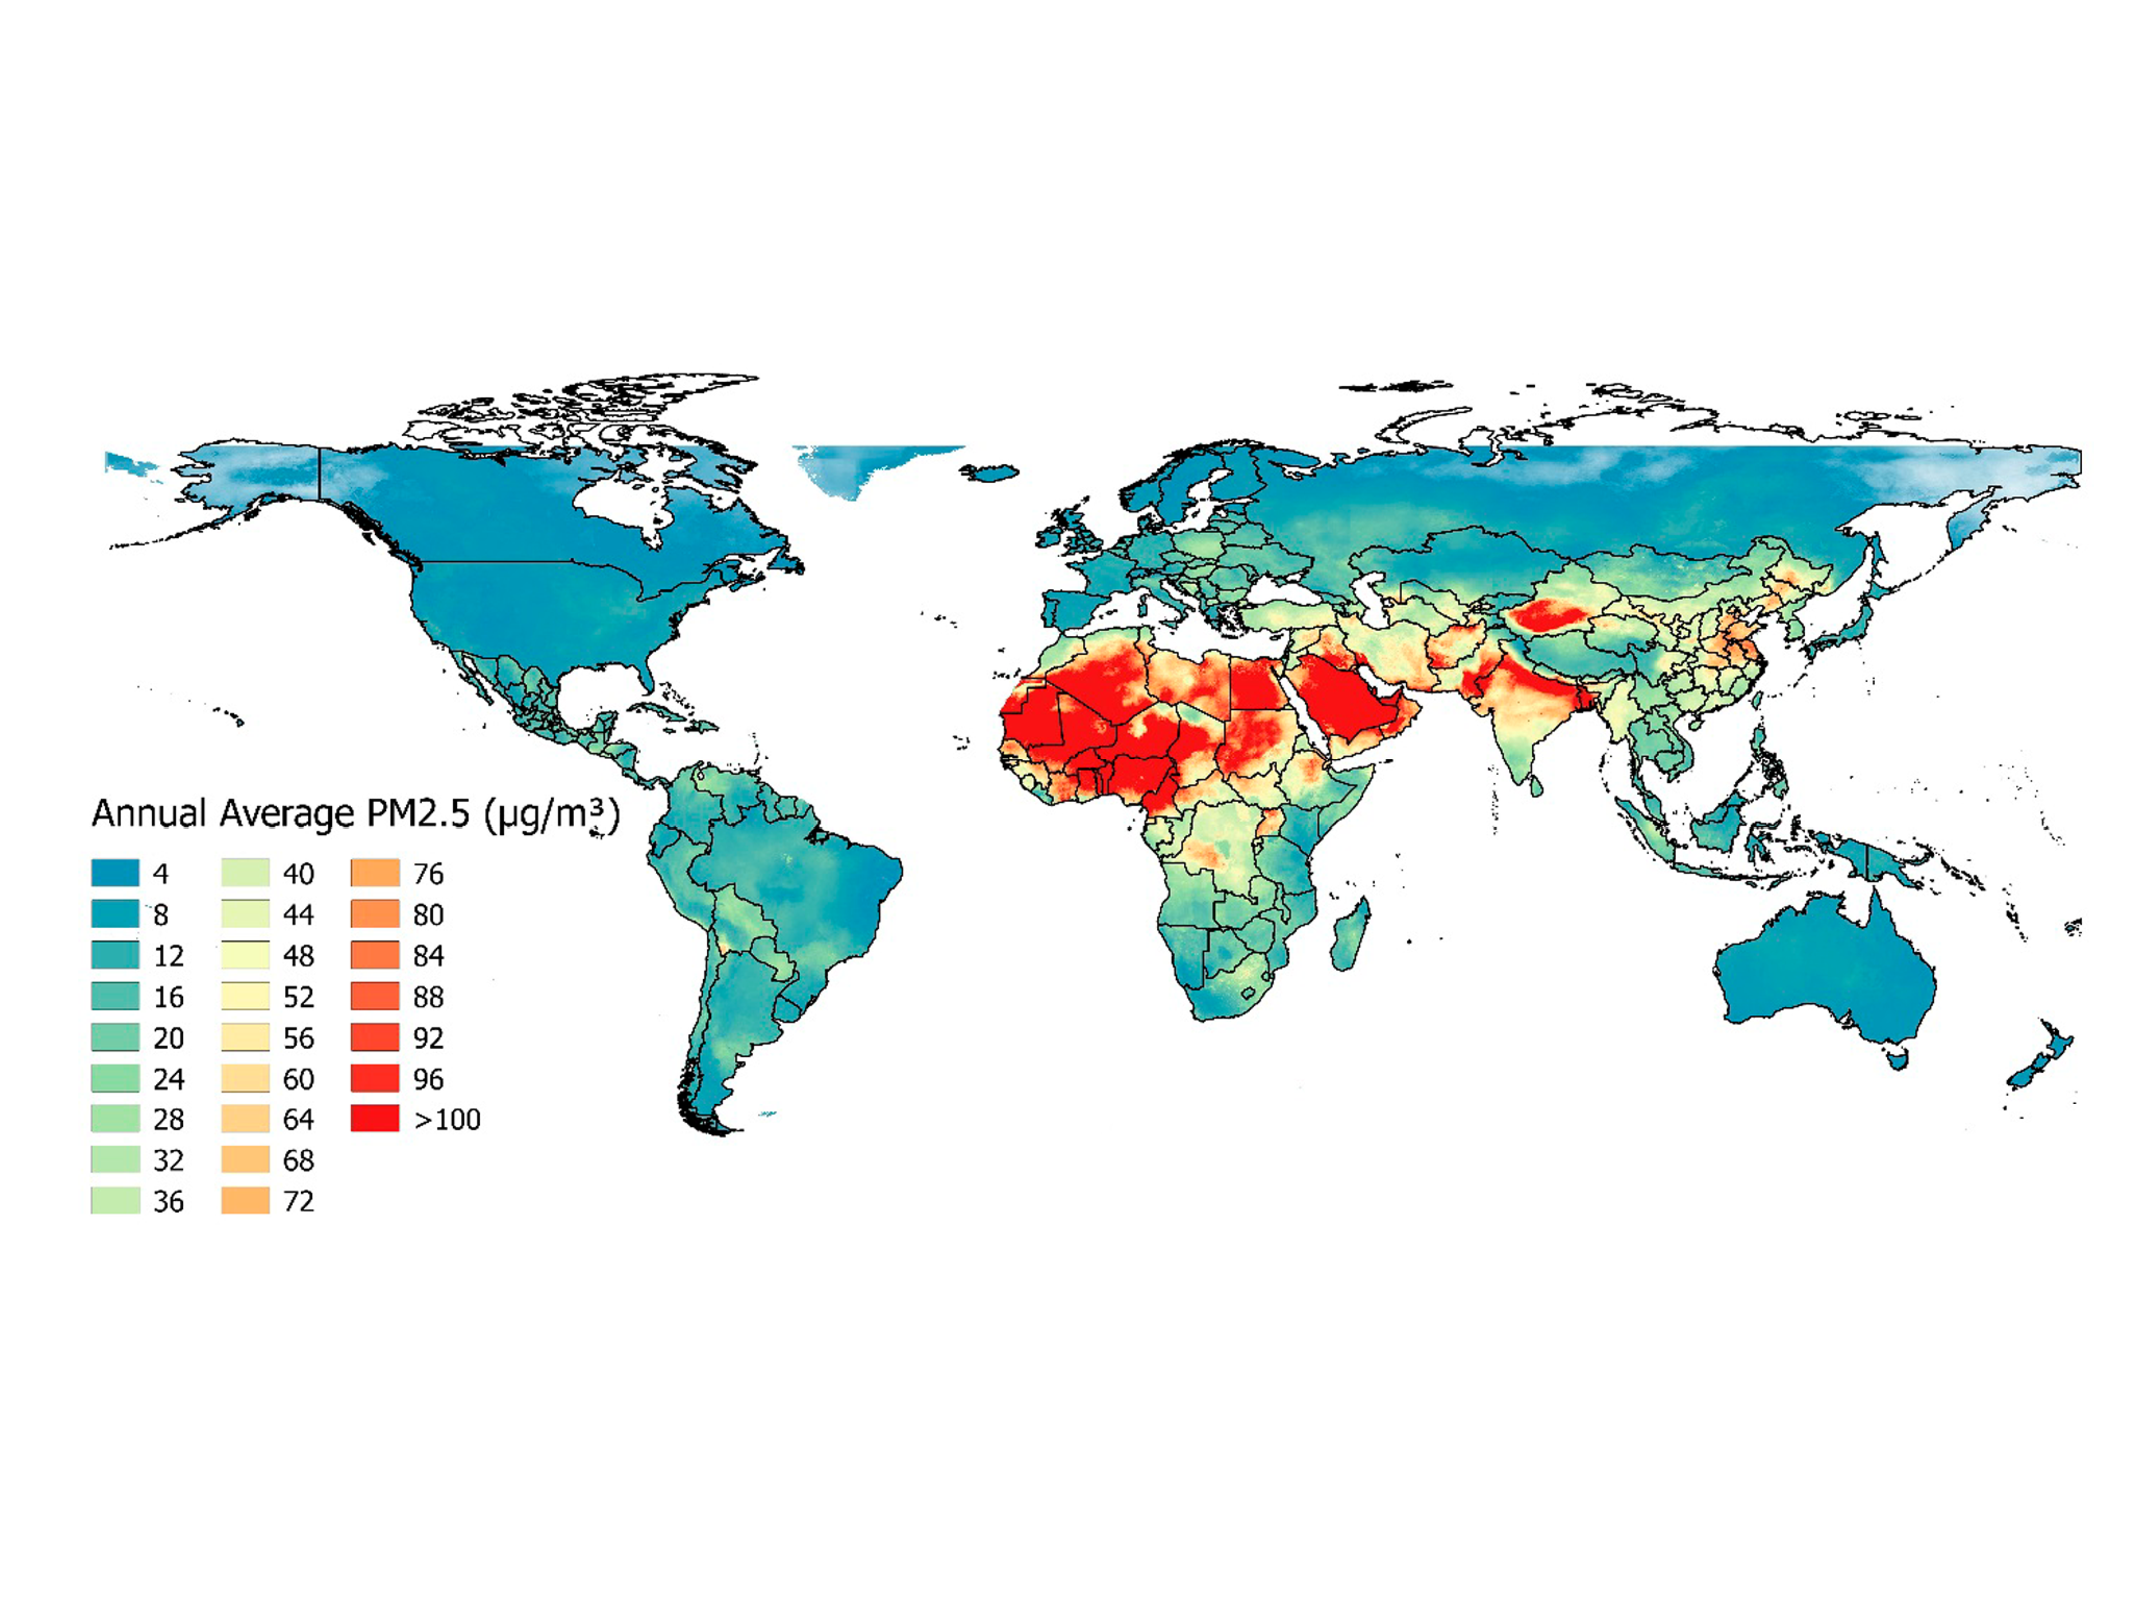
\includegraphics[width = \textwidth]{pm2_5_LUR_Shaddick.pdf}
\column{0.25\textwidth}
(From Shaddick \textit{et al} ES\&T 2018)
\end{columns}
\end{frame}

\begin{frame}{Nitrogen dioxide}

NO$_2$:
\begin{itemize}
\item Direct product of fossil fuel combustion
\item Used as an indicator for larger group of nitrogen oxides.
\item Health impact: Contributes to development of, and aggravates, asthma 
\item Environmental impact: Haze, acid rain, nutrient pollution in coastal waters
\end{itemize}

EPA Regulates NO2:
\begin{figure}
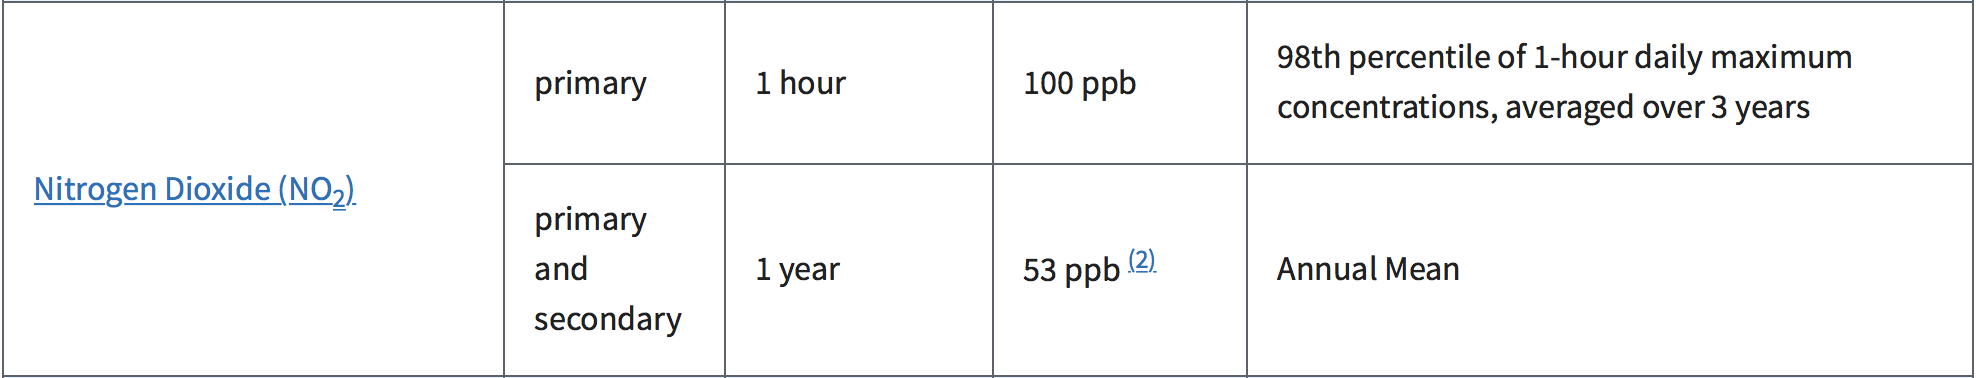
\includegraphics[width=\textwidth]{EPA_NO2_reg}
\end{figure}

\vspace{-4mm}

{\footnotesize (Primary standards are designed to protect public health.  Secondary standards are designed to address visibility, crop protection, damage to buildings, and so on.)}
\end{frame}

\begin{frame}{Novotny \textit{et al} setup}

\begin{itemize}
\item NO$_2$ concentrations are known where monitors are present.  
\item But we don't have monitors everywhere
\item Can we \textit{predict} concentrations where monitors are absent?
\end{itemize}

\pause
\begin{columns}
\column{0.5\textwidth}
\textbf{``Remote sensing'' data from satellites can be useful:}
\begin{itemize}
\item Aurora satellite ``Ozone Monitoring Instrument'' provides tropospheric NO2 column abundance (units: ppb; Called ``WRF+DOMINO'' in data set we'll work with).
\end{itemize}

\column{0.5\textwidth}
\begin{figure}
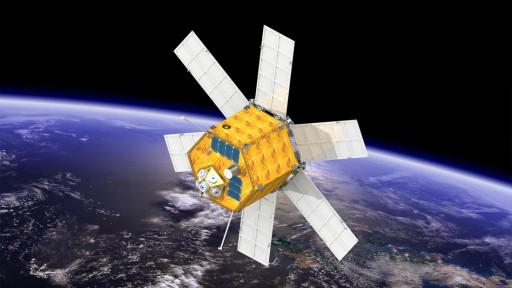
\includegraphics[width=0.75\textwidth]{aurora}
\caption*{}
\end{figure}
\end{columns}


\pause
\textbf{But!}
\begin{itemize}
\item Measurements are for entire column of air above a location, not ground-level
\item Spatial resolution is low
\end{itemize}

\end{frame}

\begin{frame}{Land use regression for NO$_2$}

\textbf{Dependent variable}: Hourly NO$_2$ concentrations from EPA sensors.

\vspace{3mm}
\textbf{Independent variables} to consider:
\vspace{-5mm}
\begin{figure}
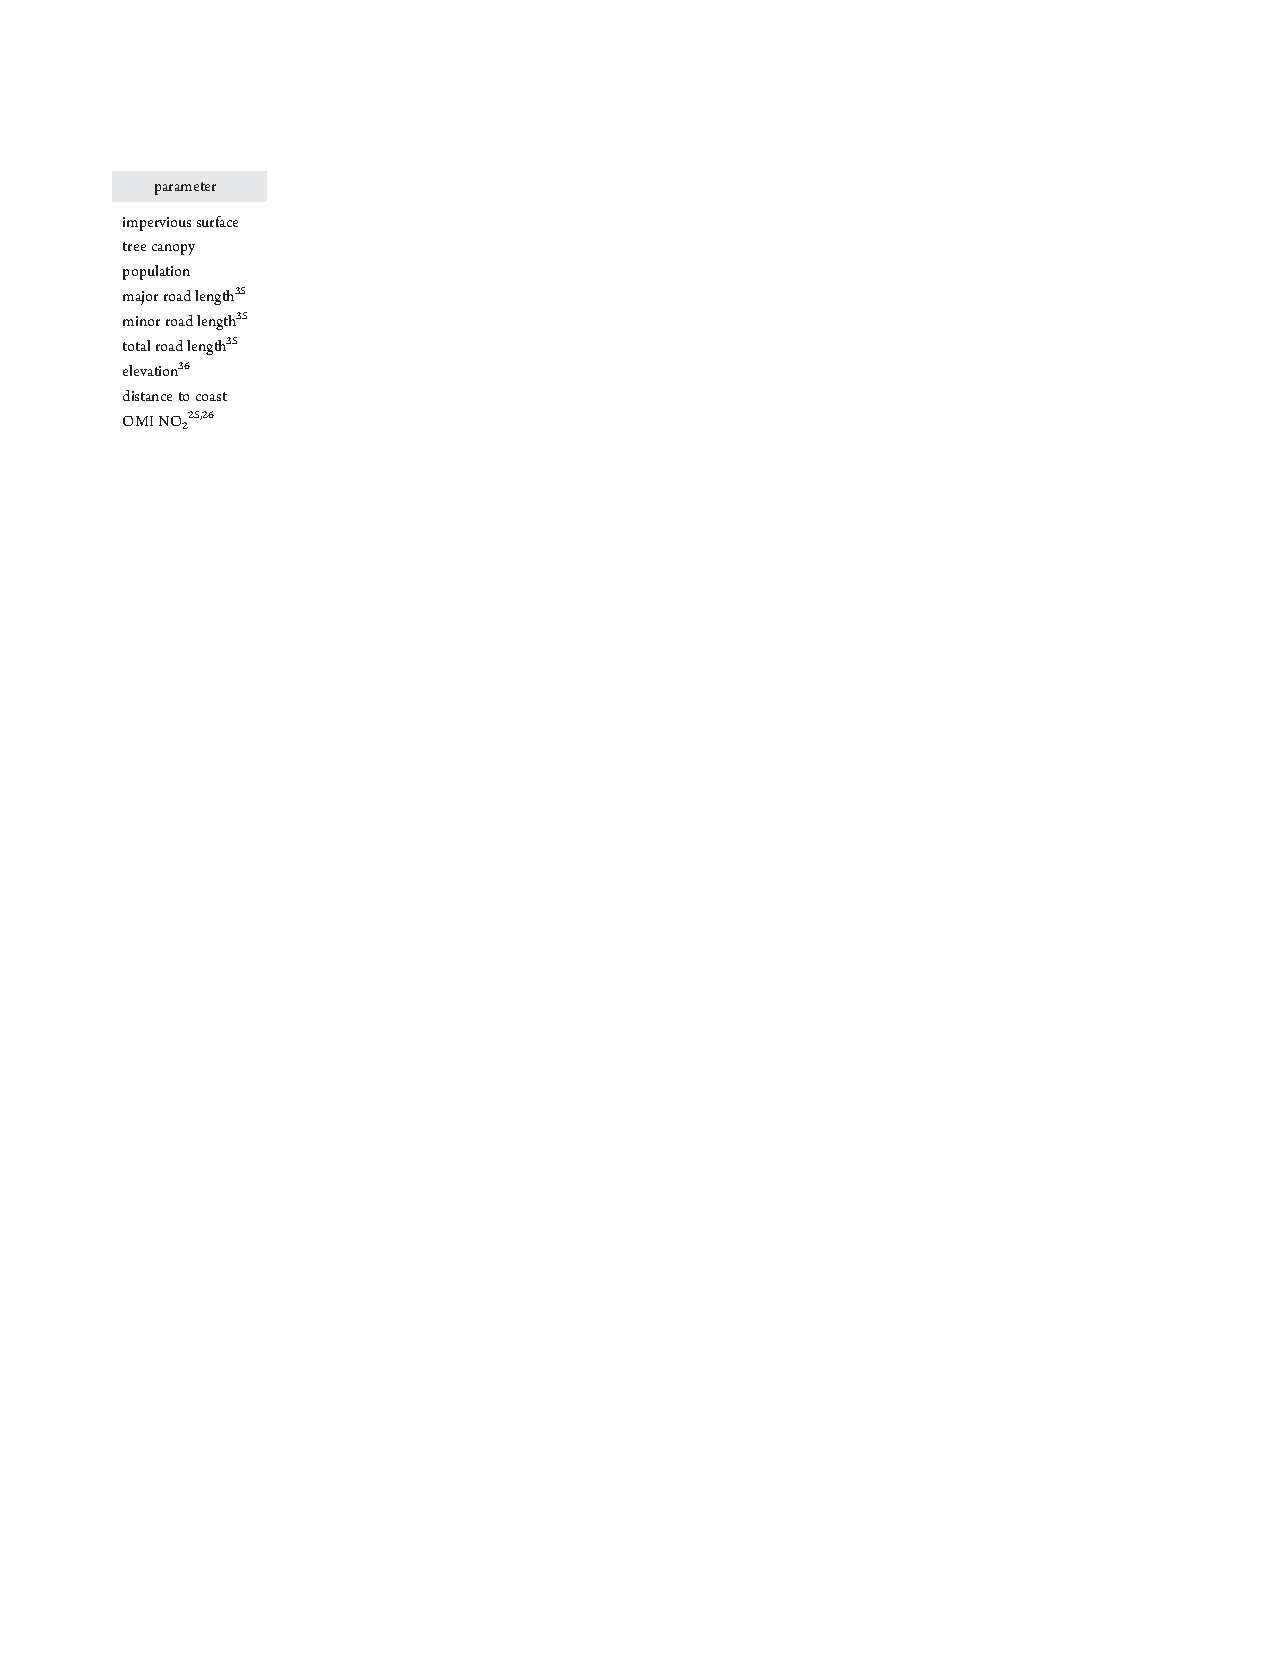
\includegraphics[height=0.6\textheight]{novotny_tab1_1}

\includegraphics[height=0.6\textheight]{novotny_tab1_2}
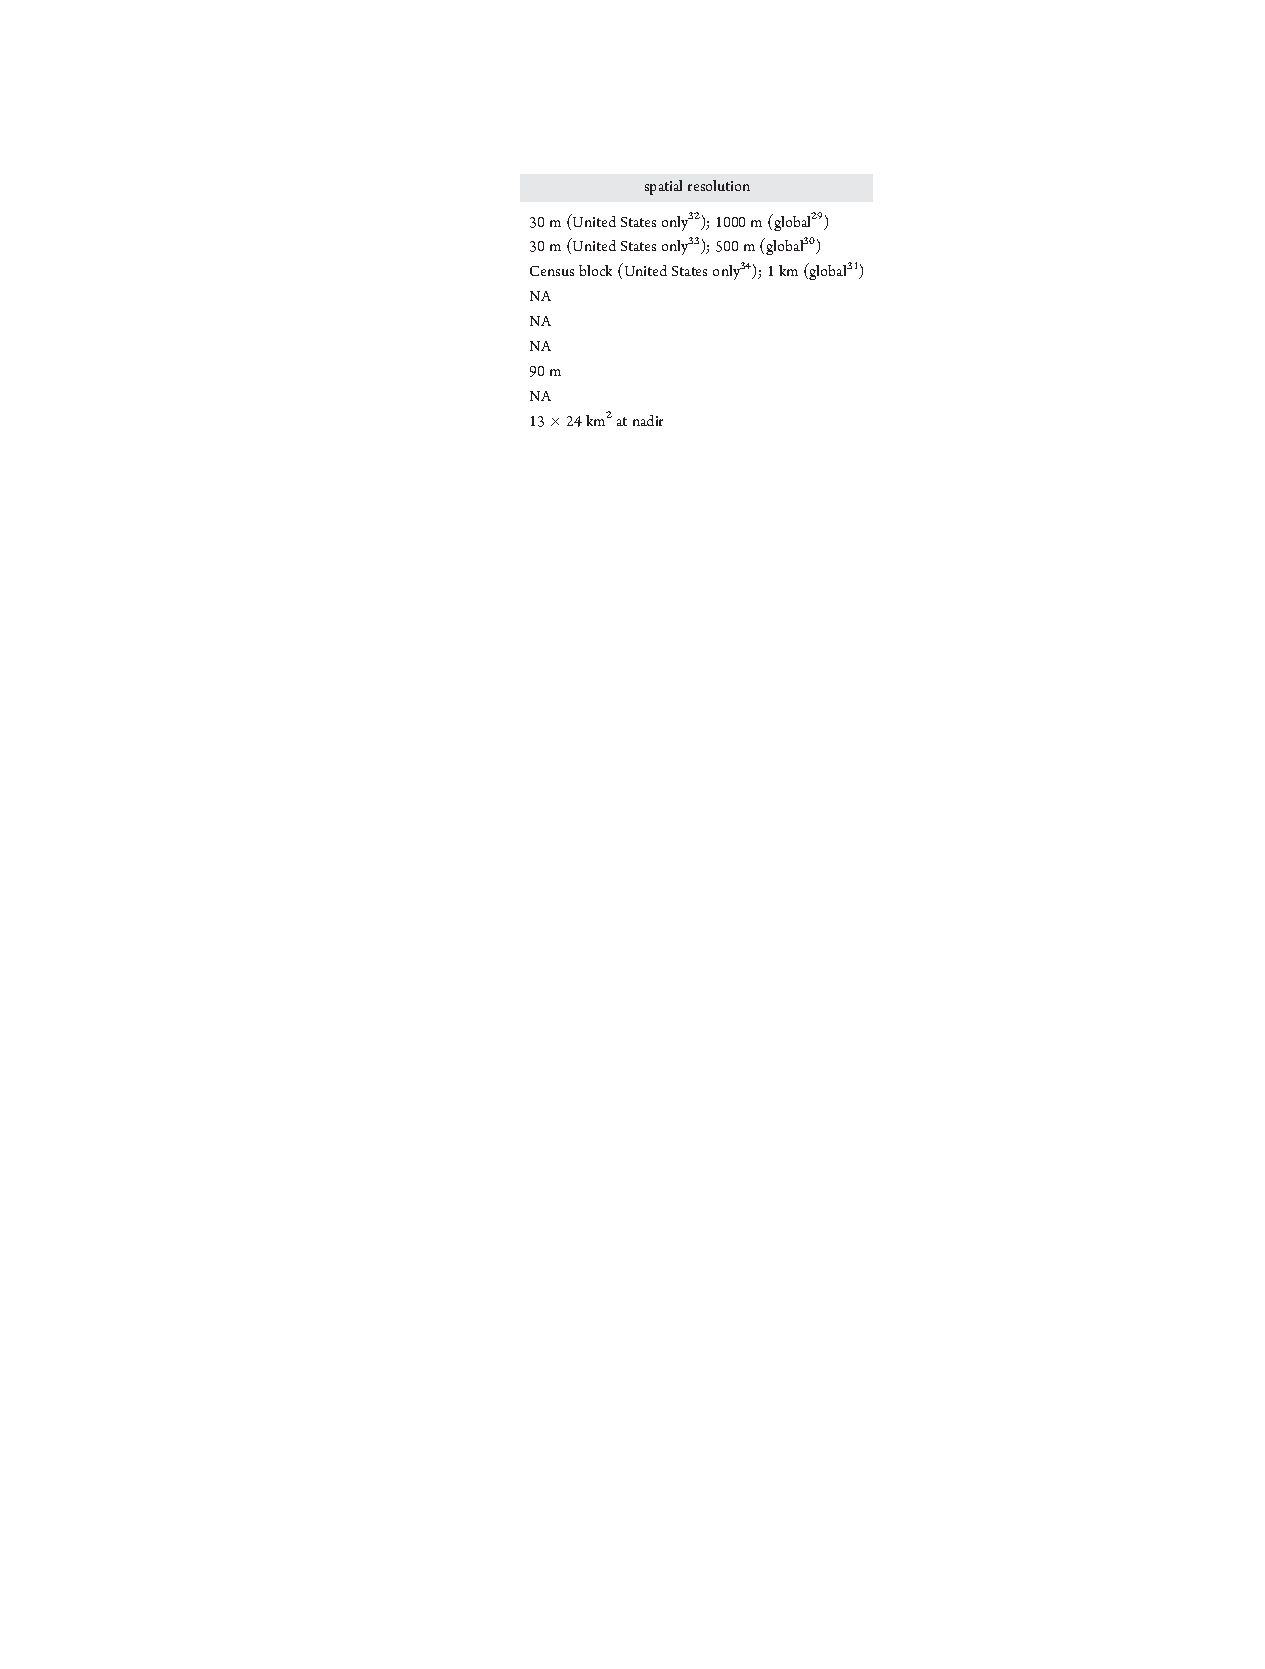
\includegraphics[height=0.6\textheight]{novotny_tab1_3}
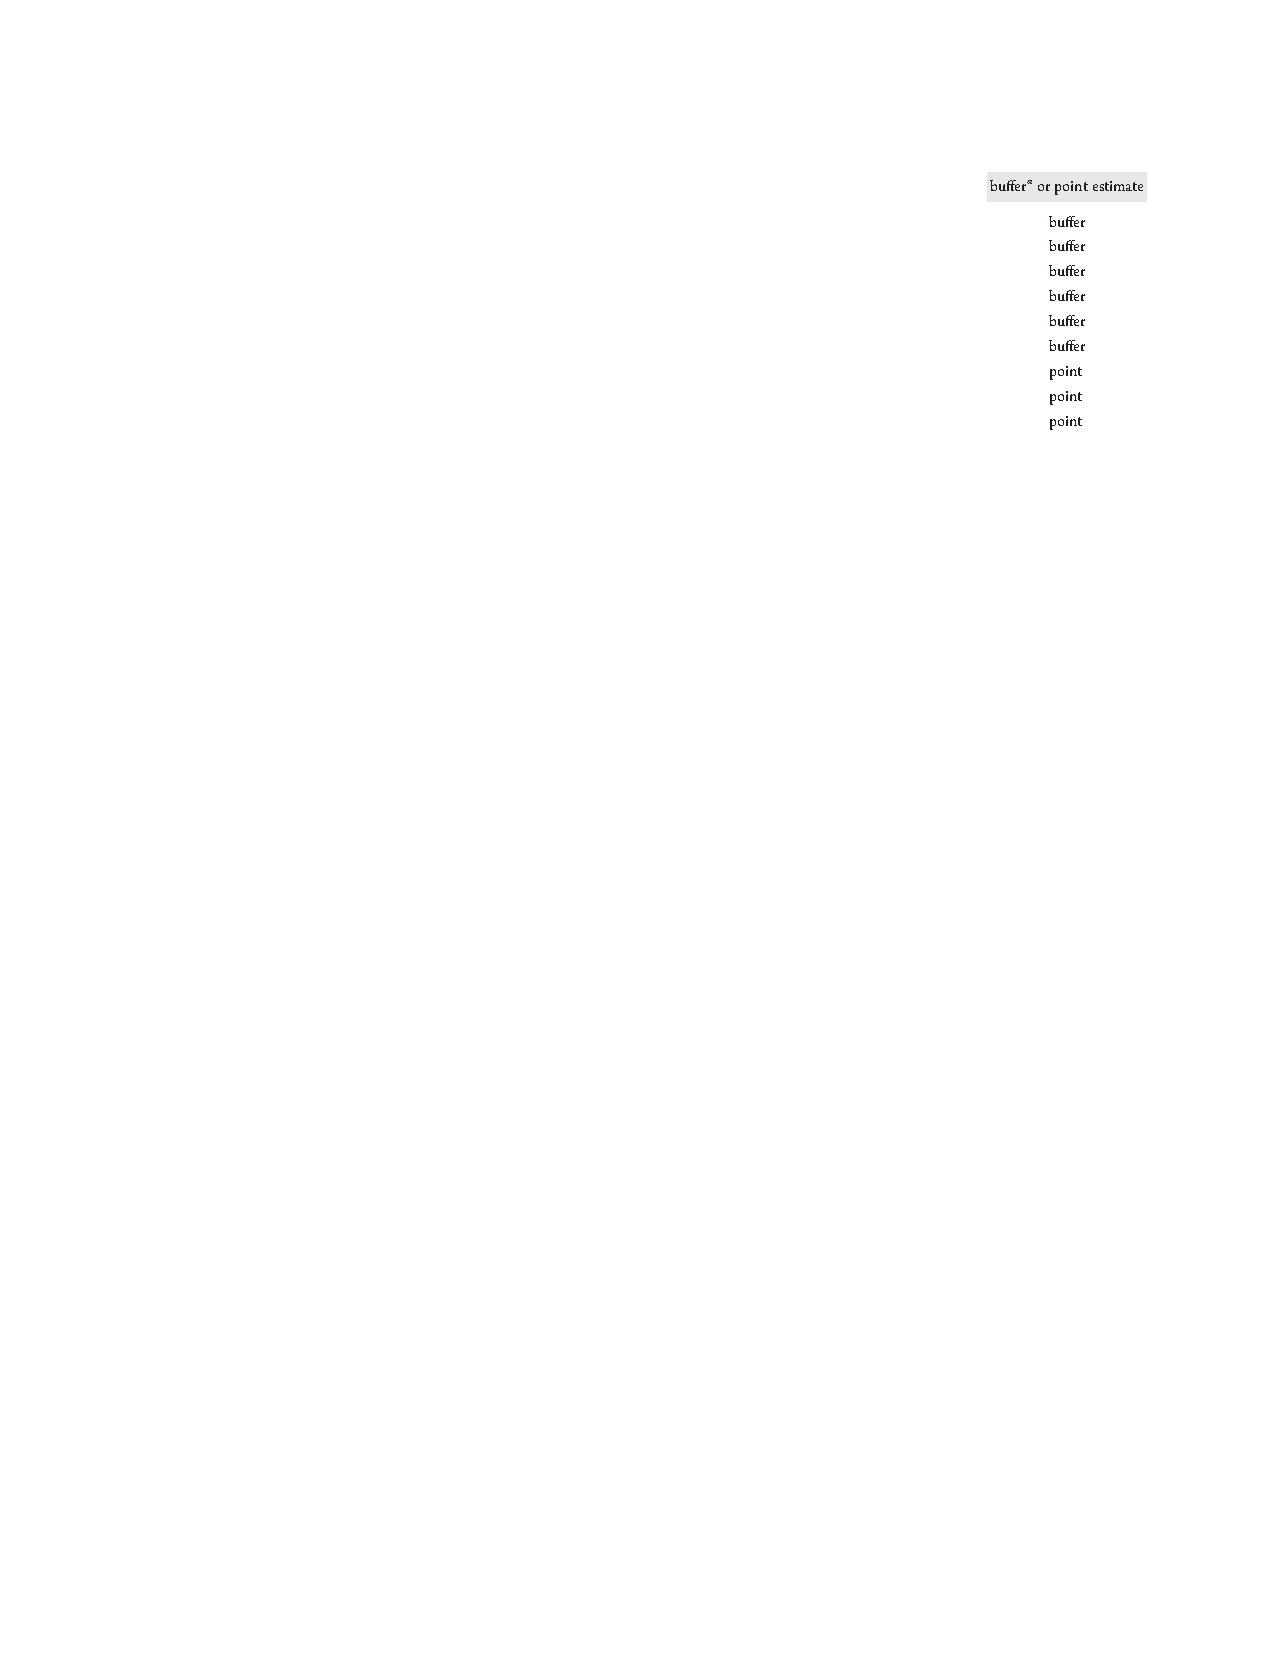
\includegraphics[height=0.6\textheight]{novotny_tab1_4}
\caption*{Novotny \textit{et al} Table 1.  }
\end{figure}

\end{frame}


\begin{frame}{}
	Let's run some linear regression models with these data.  Move over to Jupyter notebook for today's lecture.

\end{frame}

	
\end{document}


